\def\name{Example 2: Smoothly varying permeability field}

\begin{frame}{\name{}}
    \begin{figure}
        \centering
        \only<1>{%
            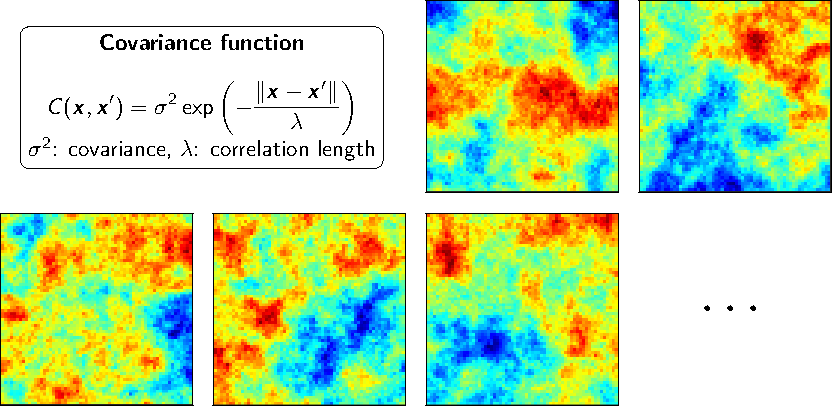
\includegraphics[width = \textwidth]{figures/example-2/perm/ex2-perm.pdf}
        }%
        \only<2>{%
            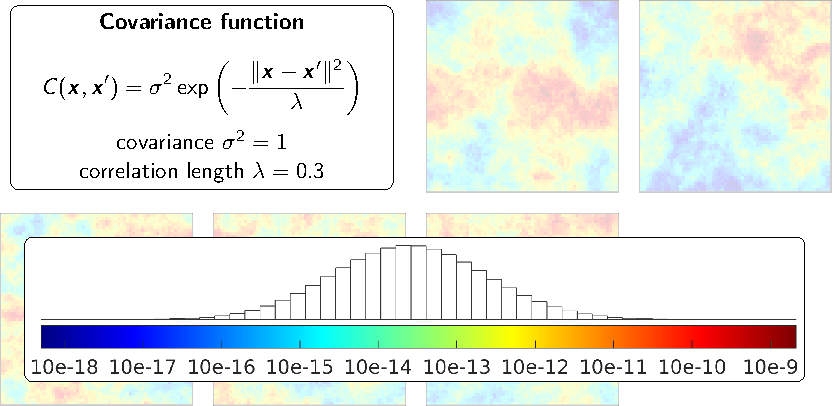
\includegraphics[width = \textwidth]{figures/example-2/perm/ex2-perm-cb.pdf}
        }%
        \only<3>{%
            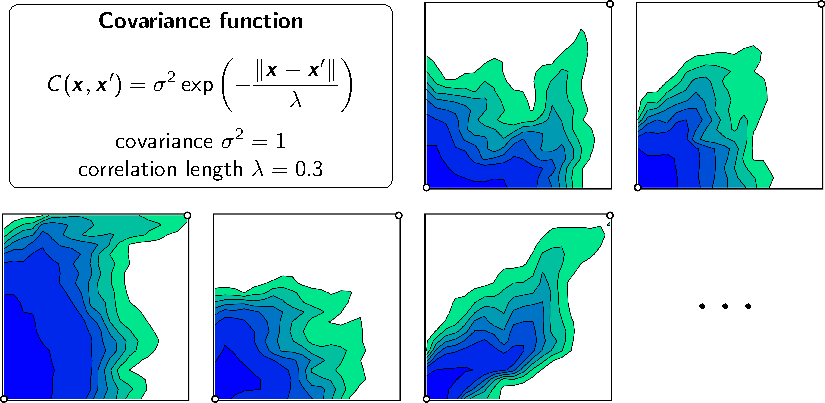
\includegraphics[width = \textwidth]{figures/example-2/sat/ex2-sat.pdf}
        }%
        \only<4>{%
            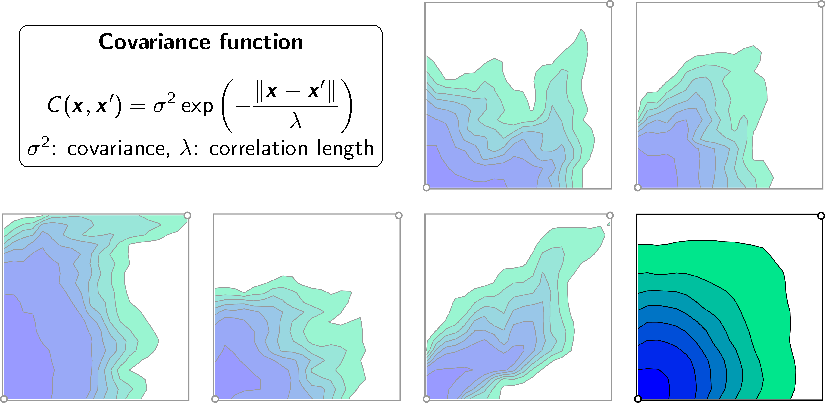
\includegraphics[width = \textwidth]{figures/example-2/sat/ex2-meansat.pdf}
        }%
    \end{figure}
\end{frame}

\begin{frame}{\name{}}
    \begin{figure}
        \centering
        \textbf{Water production rate (m$^3$/day)}
        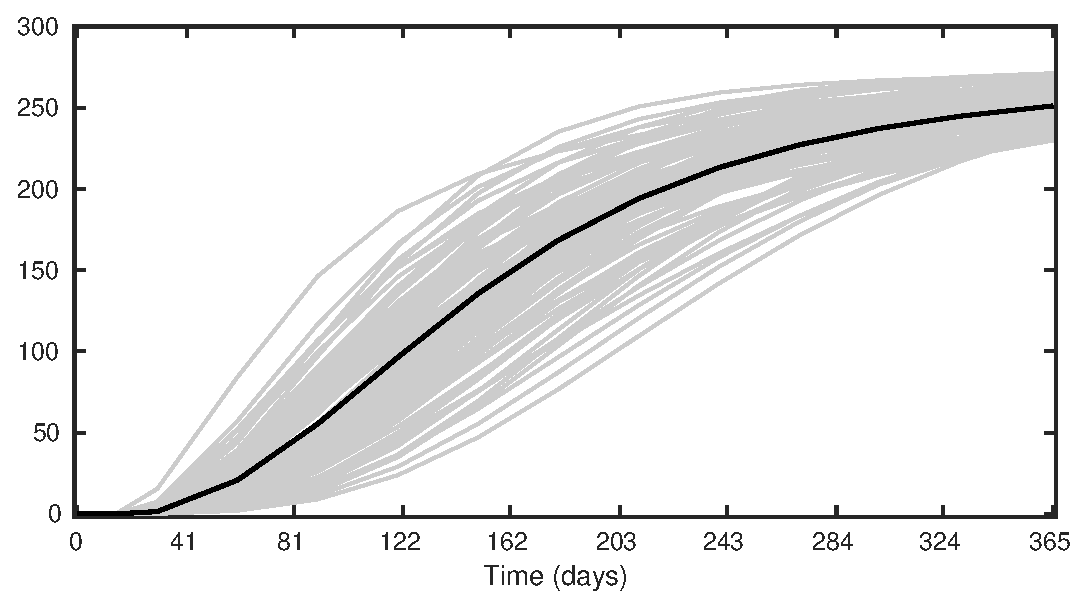
\includegraphics[width = 0.7\textwidth]{figures/example-2/water-rate.eps}
    \end{figure}
    \begin{squarelist}
        \item Monte Carlo simulation with 100 samples: Total variance $\err^\mc(q_w) = 1.1\times10^{-4}$
    \end{squarelist}
\end{frame}

\begin{frame}{\name{}}
    \begin{figure}
        \centering
        \only<1>{%
            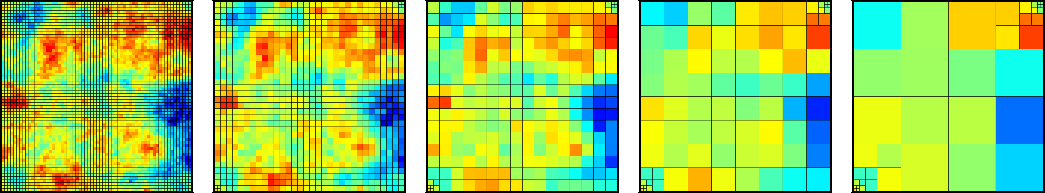
\includegraphics[width = \textwidth]{figures/example-2/permup/ex2-permup.pdf}
        }%
        \only<2>{%
            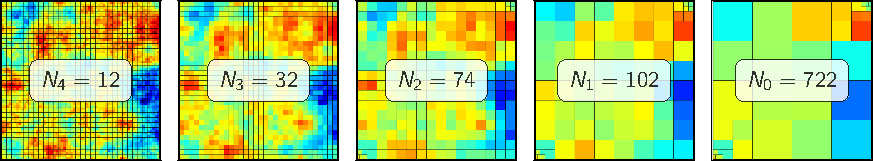
\includegraphics[width = \textwidth]{figures/example-2/permup/ex2-permup-nl.pdf}
        }%
    \end{figure}
    \begin{squarelist}
        \item<1-> Five levels with $\sim$ $4^2$, $8^2$, $16^2$, $32^2$, $64^2$ cells + refinement around wells
        \item<2-> Warmup: Run 10 samples on each level to estimate $\vara_\ell$ and $\cost_\ell$ \\
        $\rightarrow$ used to find optimal number of samples
        \begin{equation*}
            \min\, \sum_{\ell = 0}^\nlev\frac{\vara_\ell}{\nsamp_\ell} \quad \text{s.t.} \quad \cost = \sum_{\ell = 0}^\nlev \nsamp_\ell \cost_\ell \qquad \rightarrow \cost = \tol^{-2}\left(\sum_{\ell = 0}^\nlev \sqrt{\vara_\ell \cost_\ell}\right)^2, \quad \nsamp_\ell = \lambda\sqrt{\frac{\vara_\ell}{\cost_\ell}}
\end{equation*}
    \end{squarelist}
\end{frame}

\begin{frame}{\name{}}
    \begin{figure}
        \centering
        \textbf{Water production rate (m$^3$/day)}
        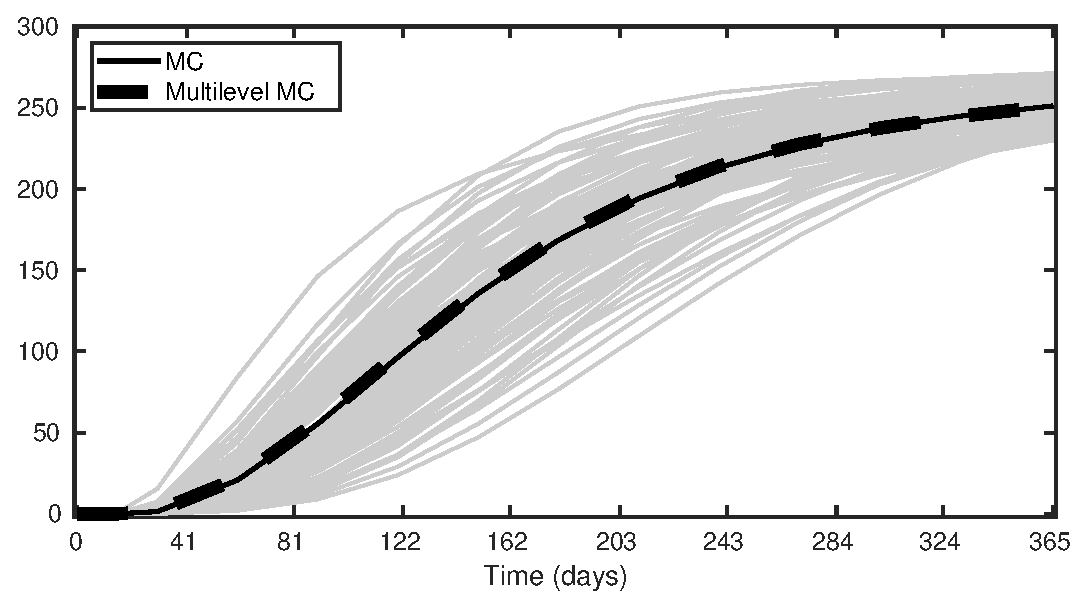
\includegraphics[width = 0.7\textwidth]{figures/example-2/water-rate-ml.eps}
    \end{figure}
    \begin{squarelist}
        \item Multilevel Monte Carlo simulation: Total variance $\err^\ml(q_w) = 1.4\times10^{-4}$
    \end{squarelist}
\end{frame}

\begin{frame}{\name{}}
    \begin{figure}
        \centering
        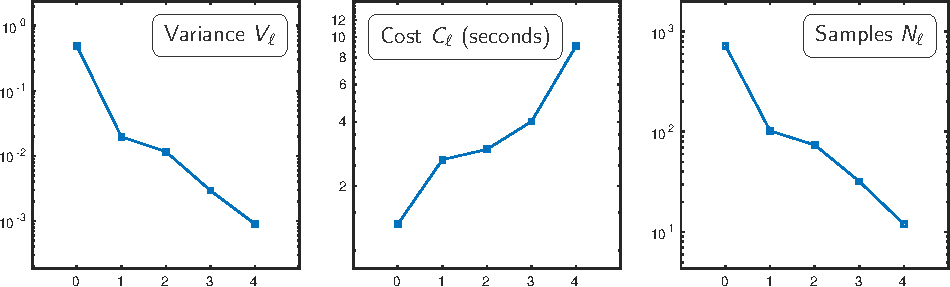
\includegraphics[width = \textwidth]{figures/example-2/statistics/ex2-statistics.pdf}
    \end{figure}
    \begin{squarelist}
        \item<1-> Total cost of Multilevel Monte Carlo: $\sum_\ell \nsamp_\ell \cost_\ell \approx \only<2>{\redtext}{1686}$ s
        \item<2-> Total cost of Monte Carlo (assuming $\cost_\nlev = $ cost of $\un_4 -\un_3$ $\approx$ cost of $\un_4$) $\approx 909$ s
    \end{squarelist}
\end{frame}